\section{Data Visualization}
\begin{itemize}
    \item See trends, clusters and patterns in data
    \item Difficult to see in raw data
    \item Detect outliers and unusual groups
    \item Validate Hypothesis/Conjecture/Theory
\end{itemize}
\textbf{Important in a Plot:}
\begin{itemize}
    \item X-Axis / Y-Axis
    \item Title
    \item Scale
    \item Dimensionality of the data 2D / 3D
\end{itemize}

\subsection{Data Analysis Libraries}
\subsubsection{NumPy}
\begin{itemize}
    \item Package for scientific computing in Python
    \item Multidimensional array object
    \item Routines for fast array operations (sorting, selecting, FFT, linalg, etc)
\end{itemize}

\subsubsection{pandas}
\begin{itemize}
    \item Built on top of NumPy
    \item Routines for accessing tabular data from files (.csv, xls, etc.)
    \item Supports 2-dimensional data (dataframe and series)
    \item Dataframes are something like database tables
\end{itemize}

\subsubsection{MatPlotLib}
\begin{itemize}
    \item Library for visualizing data
    \item Bargraphs, Histograms, Piecharts, Scatter plots, lines, boxplots, heatmaps, etc.
\end{itemize}

\subsubsection{Seaborn}
\begin{itemize}
    \item Extension of MatPlotLib, NumPy and pandas
    \item More user friendly
    \item Plots are aesthetically better
\end{itemize}

\subsubsection{Chart types}
\textbf{Line Plots}
\begin{itemize}
    \item Bivariate, Continous
    \item Recognizes trend (pattern of change)
\end{itemize}
\textbf{Bar Chart}
\begin{itemize}
    \item Used for categorical data
    \item Counting based on each category
\end{itemize}
\textbf{Histogram}
\begin{itemize}
    \item Represents the empirical distribution of a variable
    \item Automatically creates bins (interval) along the range of values
    \item Shows vertical bars to indicate the number of observations / bin
\end{itemize}
\textbf{Descriptive Statisics: Box Plots and Violin Plots}\\
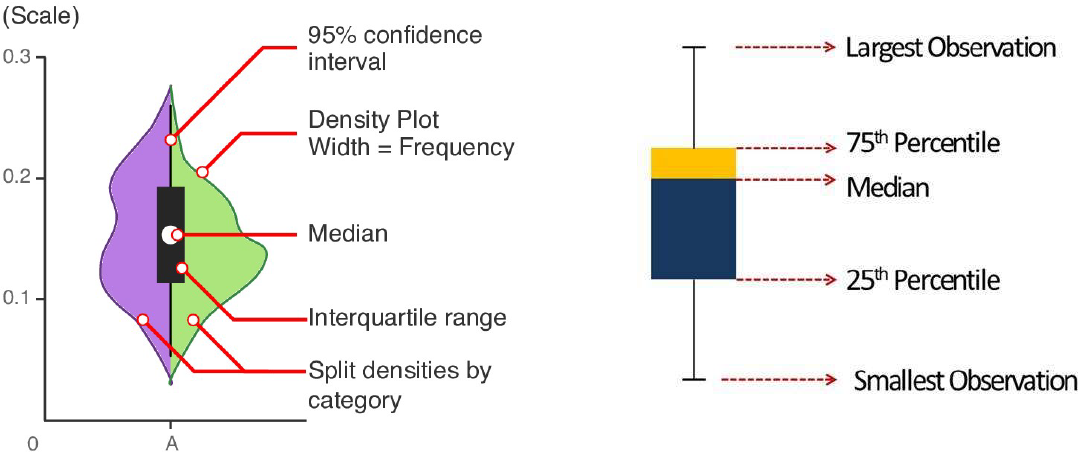
\includegraphics[width=\linewidth]{./img/descriptive_statistics.png}
\textbf{Scatter Plot}
\begin{itemize}
    \item Relationship between continous variables
    \item Helps to get an idea of the degree of correlation between variables
\end{itemize}